\documentclass[11pt,letterpaper]{article}
\usepackage[T1]{fontenc}
\usepackage{lmodern}
\usepackage{amsmath,amssymb,amsthm,mathtools}
\usepackage[letterpaper,top=.82in,bottom=.87in,left=1.0in,right=1.0in,headheight=14pt,headsep=18pt]{geometry}
\usepackage{booktabs,tabularx,xcolor,fancyhdr,microtype}
\usepackage{graphicx,tikz}
\definecolor{ink}{HTML}{202F39}
\definecolor{accent}{HTML}{195A63}
\usepackage[colorlinks=true,linkcolor=accent,urlcolor=accent,citecolor=accent,pdftitle={Planar Euclidean geometry in intuitionistic primitive recursive arithmetic}]{hyperref}
\urlstyle{same}
\usepackage{enumitem}
\setlist{topsep=4pt,itemsep=2pt,parsep=1pt}
\newtheorem{theorem}{Theorem}[section]
\newtheorem{proposition}[theorem]{Proposition}
\newtheorem{lemma}[theorem]{Lemma}
\newtheorem{corollary}[theorem]{Corollary}
\theoremstyle{definition}
\newtheorem{definition}[theorem]{Definition}
\newtheorem{remark}[theorem]{Remark}
\pagestyle{fancy}
\fancyhf{}
\fancyhead[L]{\small\sffamily\color{accent}Euclidean geometry in iPRA}
\fancyhead[R]{\small\sffamily\color{accent}\thepage}
\renewcommand{\headrulewidth}{.3pt}
\setlength{\emergencystretch}{2em}
\setcounter{tocdepth}{1}
\raggedbottom
\begin{document}
\thispagestyle{empty}
\noindent{\small\sffamily\bfseries\color{accent} FOUNDATIONS OF GEOMETRY}\hfill
{\small\sffamily 20 November 2026}\par
\vspace{13pt}
\noindent{\fontsize{27}{32}\selectfont\bfseries Planar Euclidean geometry}\par
\vspace{2pt}\noindent{\fontsize{18}{22}\selectfont in intuitionistic primitive recursive arithmetic}\par
\vspace{11pt}
\noindent\textbf{Main result.} There is a plane of finitely coded points in which
every first-order statement about betweenness and equidistance has exactly
the truth value it has in the ordinary Euclidean plane. Each statement has
a primitive recursive decision method on algebraic parameters. For a true
existence statement the method also produces a point. The equivalence with
the arithmetic translation is provable in iPRA separately for each formula.
The plane supports exact straightedge-and-compass operations and an intrinsic
reconstruction of scalar arithmetic once a unit frame is chosen.
\par\vspace{8pt}\noindent\textcolor{accent}{\rule{\linewidth}{0.8pt}}
\section{The plane and the equivalences}
\label{sec:scope}
Let $\mathcal L_{\rm pt}$ have point equality, inclusive betweenness
$B(A,X,C)$, and segment congruence $AB\equiv CD$. Variables range over
points; a line, a circle and its incidence predicates will be defined
from points. The ordinary plane means $\mathbb R^2$ in this language.
Define the arithmetic plane by $K^2$, where $K$ is the setoid of
real algebraic numbers described in Section~\ref{sec:scalar}.
A setoid consists of valid codes and an explicit equivalence relation
on codes; all predicates and operations below respect that relation.
For example, the roots isolated as $\sqrt{2}$ by two different
polynomials are the same point coordinate.

Three assertions specify the result:
\begin{enumerate}
\item \emph{Elementary equivalence.} For a closed point sentence
$\sigma$, ordinary Euclidean truth is equivalent to provability of
its arithmetic translation in iPRA. More generally, the embedding
preserves every first-order formula with parameters in $K^2$.
\item \emph{Framed coordinatization.} In the point plane itself,
an origin and two perpendicular unit directions suffice to recover
addition, multiplication, order, and both coordinates by point formulas.
Building the plane from the recovered field returns the original framed
plane up to a definable isomorphism. Without constants the frame is
a triple of parameters.
\item \emph{Construction.} Quadratic towers give exactly the coordinates
drawn by finite straightedge-and-compass constructions. Polynomial root
isolation supplies the additional points used by elementary continuity
and general first-order existential formulas.
\end{enumerate}
\noindent iPRA here has one numerical sort, symbols and defining equations
for primitive recursive functions, intuitionistic first-order logic with
equality, and induction on quantifier-free formulas. The scalar symbols
used below abbreviate total PR operations on numbers. Invalid inputs can
be sent to fixed defaults. Every bounded search has an explicit range.
The external assertion about the ordinary plane and the arithmetic proof
for each translated formula have different logical roles.

\par\vspace{7pt}
\noindent{\small\sffamily\color{accent}\textbf{Proofs and constructions}\quad
\hyperref[sec:scalar]{Scalar codes, p.~\pageref*{sec:scalar}}\quad
\hyperref[sec:qe]{Decision theorem, p.~\pageref*{sec:qe}}\quad
\hyperref[sec:synthetic]{Point axioms, p.~\pageref*{sec:synthetic}}\\
\hyperref[sec:frame-inverse]{Recovering the field, p.~\pageref*{sec:frame-inverse}}\quad
\hyperref[sec:constructions]{Constructions, p.~\pageref*{sec:constructions}}\quad
\hyperref[sec:lean]{Lean development, p.~\pageref*{sec:lean}}}
\clearpage
\section{A decidable presentation of the real algebraic field}
\label{sec:scalar}
A scalar is a finite record. We construct the records, their primitive
recursive (PR) operations and exact comparisons. In the formulas below
rationals are pairs of a signed numerator and a positive denominator.
A polynomial is a coefficient list in ascending degree with trailing
zeros removed. Polynomial coefficients in a scalar record are rational.

\subsection{Reading a scalar}
For $p=\sum_i p_iX^i$ put
\[
 M(p,R)=\sum_i |p_i|R^i,\qquad D(p,R)=M(p'',R),\qquad R\ge1.
\]
A record $(p,l,r)$ has rational $l<r$. Set
$c=(l+r)/2$, $w=(r-l)/2$, $R=1+\max(|l|,|r|)$. Its validity test is
\begin{equation}
 p(l)p(r)<0,\qquad |p'(c)|>D(p,R)w. \label{eq:intervalcheck}
\end{equation}
In particular $(X-a,a-1,a+1)$ codes a rational $a$. Invalid input
can default to the record for zero. Define $p[u,v]$ by replacing
$X^i$ by $\sum_{j<i}u^{i-1-j}v^j$ for $i>0$, and replacing $1$ by zero.
Then $p(v)-p(u)=(v-u)p[u,v]$. For $|c|,|u|,|v|\le R$,
\begin{equation}
 |p[u,v]-p'(c)|\le D(p,R)\max(|u-c|,|v-c|).
 \label{eq:divdiff}
\end{equation}
Indeed, replacing the factors of a product one at a time costs at most
$(i-1)R^{i-2}$ times the maximum displacement, and the $i$th monomial
has $i$ such products. The constant and linear cases contribute zero.
Thus \eqref{eq:intervalcheck} gives a constant sign and a positive
rational lower bound for the absolute slope on the record interval.

Bisect, retaining the half with opposite endpoint signs, or freezing
at a midpoint with $p=0$. Start with $\lceil r-l\rceil+1$ steps and
use $n$ more for precision $n$. The nested closed intervals have width
at most $2^{-n}$. Write $x$ for their value. The assertion $p(x)=0$
has a finite justification at each precision. On an interval of width
$e$ with opposite endpoint signs, the absolute value at each endpoint is
at most $M(p',R)e$ by the divided-difference identity. Frozen intervals
give exact zero. Two roots in the same record interval agree by its
positive lower slope bound.

A \emph{provisional value} is a specified PR recipe for nested rational
intervals $I_n$ of width at most $2^{-n}$, possibly with numerical
parameters. Two such recipes agree if their intervals intersect at
every equal precision. This is transitive: disjoint outer intervals have
a positive rational gap, and the intermediate interval at finer precision
cannot meet both once its width is below that gap. Strict order has a pair of separated intervals
as witness. These are schematic predicates about numbers. For example,
for inputs bounded in absolute value by $R\ge1$, multiplying two
intervals of width $e$ gives width at most $2Re$. Shifting precision
by $\lceil 2R\rceil+1$ suffices for multiplication and by one for
addition. If an interval has rational distance $b>0$ from zero, intersect
later intervals with it and invert their endpoints. Widths increase by
at most $b^{-2}$. Rational interval formulas are inclusion-preserving,
so the shifted output intervals are nested. Polynomial identities hold
for the recipes: at any requested precision use rational midpoints and
propagate errors through the expressions with these bounds. If outputs
were disjoint, they would have a rational gap, contradicted by refinement
below that gap and the rational identity. For finite expressions of
variable size fold magnitude bounds forward and required precisions
backward through the operation list. There is no quantification over
programs or sequences in this use of recipes.

\subsection{Sign and conversion to a finite record}
Suppose a provisional $x$ has a known nonzero rational annihilator $P$.
Write $P=X^k G$ with $g=G(0)\ne0$, and put
\[
 a=\min\left(\tfrac14,\frac{|g|}{8(1+\sum_{i>0}|G_i|)}\right).
\]
When $|x|\le2a$, one has $|G(x)-g|\le2a\sum_{i>0}|G_i|\le|g|/4$.
Consequently $x^k=0$ there. If $k>0$ this implies $x=0$: an enclosure
excluding zero at distance $b>0$ would give $|x^k|\ge b^k>0$.
For $k=0$ the case is impossible. Read an enclosure of width $<a$.
If it strictly excludes zero its sign is the answer with a rational
separation witness. Otherwise $|x|\le a$ and the answer is zero.
Here and throughout $n=2+\lceil1/\epsilon\rceil$ suffices for
$2^{-n}<\epsilon$.

For conversion compute the monic squarefree part $h$ of $P$ and
polynomials $U,V$ with $Uh+Vh'=1$. We have $P\mid h^{\deg P}$ over
$\mathbb Q$, so $h(x)=0$ by the power argument. Here is one bounded
way to establish these polynomial facts. Factor the primitive integer
associate of $P$ by interpolation. For degree $d>0$ select $d+1$
nonzeros of $P(j)$ among $j=0,\ldots,2d$. There are enough by
successive exact division by linear factors. An integral divisor
has a signed integer divisor of $P(j)$ at each such point. Interpolate
each tuple of possible values and test integral coefficients and exact
divisibility. Rational factorizations are covered by Gauss's lemma:
if a prime divided all coefficients of a product of two primitive
integer polynomials, reduction modulo that prime would give a zero
product of nonzero polynomials over a field, contrary to their leading
terms. At most $d-1$ successful splits are required. Take the product
of the distinct monic factors. Each is coprime to its derivative by
the degree drop in characteristic zero. Extended Euclidean division
with at most $\deg h+1$ nonzero divisions gives the displayed
B\'ezout identity. One may instead compute $h$ by dividing $P$ by
$\gcd(P,P')$ and making the quotient monic. Nonzero constant $P$
cannot annihilate a value.

Choose an integer $R>3+\max_{u\in I_0}|u|$ and put
\[
 B=\max(1,M(V,R)),\qquad L=1+D(h,R).
\]
B\'ezout gives $|h'(x)|\ge1/B$. Take $\delta=2^{-s}<1/(32BL)$
and let $c$ be the midpoint of $I_s$. Then $|x-c|\le\delta$ and
$|h'(c)|\ge1/B-L\delta$. By \eqref{eq:divdiff} every divided
difference on $[c-2\delta,c+2\delta]$, including those with $x$,
has the same sign and absolute value $>1/(2B)$. The endpoints are on
opposite sides of $x$ at distance at least $\delta$. Their $h$ values
are strictly opposite in sign. The returned record
$(h,c-2\delta,c+2\delta)$ passes \eqref{eq:intervalcheck} because its
test radius is at most $R$. Uniqueness in its interval identifies its
reader with $x$. All requested precision was computed in advance from
the given polynomial and coarse enclosure. Different records can
represent one scalar.

\subsection{Operations and equality}
For records $x_1,\ldots,x_m$ with monic annihilators $p_i$ of positive
degrees $d_i$ form the finite rational algebra
\[
 E=\mathbb Q[T_1,\ldots,T_m]/(p_1(T_1),\ldots,p_m(T_m)).
\]
Its vectors use the basis $\prod_iT_i^{e_i}$, $0\le e_i<d_i$.
Independent monic divisions in the separate variables yield the unique
representatives. Multiplication by $v$ is a rational matrix of dimension
$\prod_i d_i$. Its monic characteristic polynomial annihilates $v$,
by applying Cayley--Hamilton to the vector of $1$. Here Cayley--Hamilton
is a coefficient identity from
$(YI-A)\operatorname{adj}(YI-A)=\det(YI-A)I$. Multiply the coefficient
identities on the left by the corresponding powers of $A$ and sum to
obtain cancellation. Determinants can use their finite permutation
sums. Substitution $T_i\mapsto x_i$ preserves reductions because each
$p_i(x_i)=0$, irrespective of relations among the different $x_i$.

Use $v=T_1+T_2,T_1-T_2,T_1T_2,-T_1$, respectively, for an annihilator
for each ring operation. Compute the provisional value with interval
arithmetic and convert as above. For a nonzero input use its separated
enclosure to invert, and the reversed polynomial $X^{\deg p}p(1/X)$
as annihilator. Inversion at zero is totalized by zero. Compare two
records by determining the sign of their difference. It is zero exactly
when the two readers agree: nested input pairs that intersect at every
precision have all interval differences containing zero, while a pair
separated at some precision remains separated under refinement. Thus
record equality is a PR setoid relation. The ordered-field laws hold
modulo this equality by the rational identities of the interval recipes.
In detail, trichotomy comes from the sign test, translation preserves
signed separation after a sufficiently accurate read of the common
summand, and positive lower bounds $b,c$ give the product lower bound
$bc$. Denote the resulting field by $F$.

\subsection{Polynomial IVT and exhaustive root lists}
For a nonconstant monic $f(Z)=Z^n+\sum_{i<n}x_i Z^i$ over $F$, take
the algebra $E$ just described and set
$\widetilde f(Z)=Z^n+\sum_{i<n}T_iZ^i$ (index the generators from zero).
Form the rational matrix of multiplication by $Z$ on
$E[Z]/(\widetilde f)$. Its monic characteristic polynomial $H(Y)$,
of degree $n\prod_i d_i$, satisfies
\begin{equation}
 f(y)=0\quad\Longrightarrow\quad H(y)=0
 \label{eq:elimroots}
\end{equation}
even for a provisional value $y$. Indeed $H(Z)=0$ in the finite
algebra, and evaluation preserves every defining relation when
$T_i\mapsto x_i$ and $Z\mapsto y$. Extra roots of coefficient
annihilators do not affect this implication.

For $s<t$ and $f(s)f(t)<0$, substitute $s+(t-s)X$, trim leading
zeros by the field comparison and make the result monic. Its degree
is positive. Bisect $[0,1]$. Each midpoint is rational and its polynomial
sign is computable in $F$. Freeze at an exact root. After $k$ steps the
width is at most $2^{-k}$. The provisional $y$ is a zero: the endpoint
sign argument for reading a record still applies, using a rational
upper bound on $M(f',1)$ for the transformed polynomial, obtained from
its coefficient enclosures. By \eqref{eq:elimroots} conversion returns
a record of $y$. Undo the substitution. The result is strictly interior
by endpoint nonvanishing and trichotomy. Positive scalars therefore
have positive square roots (apply this result to $X^2-b$ on $[0,b+1]$).
Odd-degree polynomials have zeros by leading-term dominance at
$\pm R$ for $R>1+\sum_{i<n}|f_i|$ after monic normalization. This
establishes the positive-square and odd-degree-root axioms of a real
closed field and the polynomial intermediate value property.

There is also a uniform PR list of all distinct roots in increasing order.
Return the empty list for a nonzero constant and flag the zero polynomial
as everywhere zero. Otherwise form $H$ by \eqref{eq:elimroots} after
monic normalization and take its monic squarefree part $h$. Choose
an integer $R>2+\sum_{i<\deg h}|h_i|$. All roots of $h$ are strictly
inside $[-R,R]$ by leading-term dominance. Compute $B,L$ as in the
conversion proof with radius $R+1$, and partition $[-R,R]$ by a dyadic
mesh $\delta<1/(32BL)$. Record every grid zero and every open cell
with opposite endpoint signs. Recover a provisional root in a crossing
cell by rational bisection and convert it. For any $F$ root $z$ of $h$,
locate it among the grid points by field comparisons. If it is in an
open cell, the B\'ezout bound at $z$ and \eqref{eq:divdiff} give constant
slope sign and absolute slope $>1/(2B)$ throughout that cell. Its endpoint
signs must be opposite, and the recovered root equals $z$. The same
estimate at a grid zero excludes another zero in either neighboring open
cell. This gives the complete ordered list for $h$. Keep only those
entries satisfying $f(z)=0$ in $F$. Every $F$ zero survives by
\eqref{eq:elimroots} and divisibility $H\mid h^{\deg H}$. Externally
the same grid argument over the ordinary reals identifies $F$ with all
real algebraic numbers. Every record has its real zero by bisection
and every real zero of a rational polynomial is found by the grid.

\subsection{Induction and uniformity}
Integers, rationals, coefficient lists, interval endpoints, permutations
and matrix tables are number codes. For example use $0$ for the empty
list and $\operatorname{cons}(a,b)=2^a(2b+1)$. Decoding, length and
indexed access are bounded by the list code. Builders enlarge codes by
primitive recursion. Euclidean division has degree fuel, determinants
and interpolation tuples range over the finite sets described above,
and the grid has $2R/\delta$ cells. A bisection calling a previously
defined PR field-sign operation is primitive recursion. Computing a field
sign uses rational interval reading and the scalar arithmetic, with no
calls to the algebraic-coefficient root finder. A failed bounded search
on malformed data returns a fixed default record or list. The proofs
above exclude that branch on valid arguments.

For the induction restriction, the signs in an initial portion of
a grid are a bounded Boolean fold. Polynomial division retains the
quotients, so its invariant is an identity of concrete coefficient
vectors. Cofactor identities are equalities of finite rational sums,
with cancellation paired by interchanging two indices. Width bounds
and endpoint signs in a bisection are rational inequalities or Boolean
field tests at the current stage. The product expansion in
\eqref{eq:divdiff} uses a finite telescoping sum. Factorization and
B\'ezout witnesses are coefficient vectors, and candidate divisors are
tested in bounded lists. For identities of provisional values, fix an
output precision before the calculation, propagate the rational bounds
through the finite operation list and apply induction to rational
data. For instance, in the power argument an enclosure allegedly
separated from zero supplies its own rational gap and hence a
precision that distinguishes its power from zero. Generalizing over
the requested precision is a logical inference after the finite
calculation. Induction over a property universally quantified over
precisions, and a universal evaluator for PR programs, are both
unnecessary.

For other constructions of PR field presentations see V.~Selivanov and
S.~Selivanova, \emph{Primitive recursive ordered fields and some
applications} (\url{https://arxiv.org/abs/2010.10189}). For a constructive
formalization see C.~Cohen, \emph{Construction of real algebraic numbers
in Coq} (\url{https://perso.crans.org/cohen/papers/realalg.pdf}).

\section{Deciding a formula and extracting its witnesses}
\label{sec:qe}
Write $K$ for the coded field of the preceding construction. We give the
elimination argument because a decision procedure proved terminating in a
stronger theory would by itself give insufficient information about iPRA.
The geometric atoms are point equality, equidistance and inclusive
betweenness. Translate them respectively into component equality,
equality of squared distances, and
\[
  [C-A,X-A]=0\ \land\ (X-A)\cdot(X-C)\le0.
\]
Section~\ref{sec:synthetic} proves the last equivalence. Relativize numerical
quantifiers to valid codes, use field equality on representatives, replace
each point binder by two scalar binders, and commute the translation with
each intuitionistic connective. This is the interpretation $\varphi^\#$.
Induction on each fixed formula shows that replacement of a parameter by an equal code preserves its interpretation: this holds for atoms, commutes with the connectives, and holds for each admissible assignment under a binder. We next give a quantifier-free ordered-ring formula for each such
formula before interpreting its scalar variables by codes.

\subsection{Counting a sign at real roots}
For a nonconstant squarefree univariate $D$ and any $W$ in $K[T]$, define
\[
   Q_D(W)=\sum_{D(r)=0}\operatorname{sgn} W(r),
\]
with each distinct root counted once. We show how to compute it using
only coefficient arithmetic and sign tests. Reduce $D'W$ modulo $D$;
if the remainder is zero the answer is zero. Otherwise cancel the gcd
of the remainder and $D$, dividing both by the same monic polynomial,
to obtain coprime $B,A$ with $B/A$ the reduced proper fraction. Form
\[
 S_0=A,\quad S_1=B,\qquad S_{i+1}=-\operatorname{rem}(S_{i-1},S_i)
\]
until just before the zero remainder. The last entry is a nonzero
constant. At $+\infty$ record the sign of each leading coefficient;
at $-\infty$ multiply it by $(-1)^{\deg S_i}$. Let $V_+,V_-$ be the
numbers of variations between consecutive signs. Then
\begin{equation}
                  Q_D(W)=V_- - V_+.                 \label{eq:query}
\end{equation}
Indeed, signs are constant between consecutive roots of the product
of the $S_i$ by polynomial intermediate value. Neighboring entries
have no common root, by the Euclidean identities and coprimality.
At a zero of an interior entry the neighboring values are opposite
by the signed remainder identity. Its two adjacent edges have one
variation in total on either side. Several interior entries may vanish
at the same point; their pairs of edges are disjoint. The final entry
has no root. At a root $r$ of the first entry, its root is simple,
and the first edge loses one variation if $B(r)/A'(r)>0$ and gains one
if it is negative. To check this, write $A=(T-r)A_1$, where
$A_1(r)=A'(r)$; sufficiently close to $r$, $A_1$ and $B$ have their
signs at $r$. For a polynomial $g$ with $g(r)\ne0$ this last assertion
has an explicit bound: write $g(r+h)-g(r)=\sum_{j\ge1}c_jh^j$ and take
$|h|<\min(1,|g(r)|/(1+\sum|c_j|))$. Edge changes telescope.
At an uncancelled root of $D$, the coefficient of $1/(T-r)$ in
$D'W/D$ is $W(r)$, as follows from $D=(T-r)D_1$ and $D'(r)=D_1(r)$.
Removing the polynomial part or a common factor preserves this coefficient.
Cancelled roots have $W(r)=0$. This proves~\eqref{eq:query}, including
the case that there are no roots. Signs on the tails have the claimed
values by dominance of the leading term; one may use
$|T|>1+\sum_{j<d}|a_j/a_d|$. For a constant $D\ne0$ set all queries to zero.

For a list $f_1,\ldots,f_m$ and a prescribed sign vector
$\sigma\in\{-1,0,1\}^m$, its count among the roots of $D$ is computed
without comparing unknown roots. Use the three integer polynomials
\[
 I_0(z)=2(1-z^2),\qquad I_{+}(z)=z^2+z,\qquad I_{-}(z)=z^2-z .
\]
On a sign input, each is twice the indicator of its named sign. Expand
$\prod_j I_{\sigma_j}(Z_j)=\sum_e c_e Z^e$. Then the desired count times
$2^m$ is
\begin{equation}
             \sum_e c_e\, Q_D\Big(\prod_j f_j^{e_j}\Big).      \label{eq:counts}
\end{equation}
This follows by expansion at each distinct root and multiplicativity of
sign, with $z^0=1$ also at zero. Positivity of this integer is the
test for occurrence.

\subsection{One scalar quantifier}
Specialize all other variables to any fixed parameter tuple for the
moment. Given the polynomials occurring in a quantifier-free formula
$\theta(T)$, first drop the constants, retaining their signs. Let $P$ be
the monic squarefree part of the product of the rest. If none remain,
one sample $T=0$ suffices. For squarefree extraction over $K$, divide by the gcd with the derivative. At a proposed root $r$ divide repeatedly by $T-r$, with degree fuel, to write the original product as $(T-r)^e U$, $U(r)\ne0$. For $e>0$ its derivative has multiplicity $e-1$ there. The gcd has the smaller multiplicity, by common divisibility and the B\'ezout identity. Thus extraction preserves every root and makes it simple. When a nonconstant polynomial remains, the signs attained anywhere on
the line are precisely those among the following finite tests:
\begin{enumerate}
\item the signs on the left and right unbounded tails;
\item sign vectors occurring at a root of $P$;
\item sign vectors occurring at a root of the squarefree part of $P'$
(omit this test for a constant derivative).
\end{enumerate}
Indeed a sign cannot change inside a root-free interval. For consecutive
roots $a<b$ of $P$, simplicity gives
$\operatorname{sgn}P'(a)=-\operatorname{sgn}P'(b)$: factor $T-a$ at the
left and $T-b$ at the right and use the common interior sign. The
local bound in the preceding paragraph supplies actual one-sided test
points, using also half the gap. Polynomial intermediate value applied
to $P'$ gives a root strictly between $a,b$. Thus the list samples
every bounded open cell as well as all singleton cells. If $P$ has at
most one root, the same proof uses only the singleton and tail cases.
Evaluate the propositional formula on these signs. Existential truth is
equivalent to at least one true evaluation. For witnesses in $K$, use its
sorted root lists directly, including midpoints for bounded intervals and
the extreme roots shifted outwards by one for unbounded intervals
(use zero if there are no roots). An inhabitant and, in the universal
case, a counterexample when it fails, are both primitive recursively
obtainable. This also justifies using Boolean implication for this
specific decidable matrix in intuitionistic logic.

To remove the specialization, run the same coefficient algorithm
symbolically, splitting into three branches at each sign test on the
parameters. In particular test leading terms before dividing, discard
an identically zero specialized polynomial on the appropriate branch,
and truncate to the actual degree. On any branch every scalar coefficient
computed is a rational function $p/q$ in the parameters with $q\ne0$
along that branch. Its sign is the sign of $pq$, since $q^2>0$.
Thus every guard is a polynomial sign formula. The disjunction of the
guards for the accepting leaves is a quantifier-free formula in the
parameters. Keep coefficient pairs formal even on inconsistent branches. A division by $a/b$ is performed symbolically only on the branch guarded by $a\ne0$; inductively all denominators on a realized branch are nonzero. No branch-feasibility oracle is needed.
Symbolic root extraction is unnecessary: counts and tails use only
coefficient arithmetic. This is a specialization-safe elimination even
where a discriminant or several leading coefficients vanish.

Here are bounds on generating the tree. If the original list has $m$
polynomials of degree at most $d$ in $T$, put $s=1+m(d+1)$.
The product has degree below $s$, the squarefree parts and their
derivatives have degree below $s$, and all test products in
\eqref{eq:counts} have degree at most $2md$. A Euclidean gcd or signed
remainder chain uses at most the initial maximum degree plus two
divisions, each a loop of at most that degree plus two cancellations.
Polynomial products use finite convolutions. There are $3^m$ target
patterns and at most $3^m$ monomials per expanded indicator product.
For precision, a finite program with just these bounded loops can be
unrolled by primitive recursion on their displayed bounds. For every
scalar operation the size of a pair of numerator/denominator expression
trees of size at most $b$ is bounded, for instance, by $8(b+1)$ for
each new tree if expressions remain unexpanded. Record a three-way
branch by duplicating the remaining program at most three times per
test. Iteration of these size bounds along the unrolled program, or
construction of its whole ternary tree by recursion on its instruction
budget, is primitive recursive. Expansion and collection of the resulting
polynomials are finite folds on their syntax. Repeating one-variable
elimination from the innermost binder out is iteration of a fixed PR
transformation on coded syntax, hence PR even with formula length an
input. Efficiency is immaterial to the proof.

\begin{theorem}[Elementary equivalence and arithmetical derivability]
\label{thm:transfer}
For each fixed first-order point formula $\varphi(\bar P)$ there is
a PR test $b_\varphi$ such that iPRA proves, on valid parameter codes,
\[
                  \varphi^\#(\bar P)\ \longleftrightarrow\
                  b_\varphi(\bar P)=1 .
\]
The test takes only the values zero and one. For algebraic parameters
the standard real plane agrees with this test. In particular, for a
closed sentence $\sigma$ the following are equivalent: its truth in
the ordinary Euclidean plane; its truth in the coded plane in the
standard naturals; and $\mathrm{iPRA}\vdash\sigma^\#$.
\end{theorem}
\begin{proof}
For the internal assertion use the root and order theorems of the scalar
construction and the elimination calculation above. For each fixed formula,
structural induction here is on the external formula. At an existential
step the accepting branch has a sample witnessing the matrix, and the
rejecting branch excludes every sample and hence every candidate. At a
universal step reject with the constructed counterexample or prove the
matrix for an arbitrary input by its realized sign cell. Equivalently,
one may eliminate $\neg\exists T\,\neg\theta(T)$ after this argument
establishes the equivalence; the witness step matters intuitionistically.
Boolean cases for conjunction, disjunction and implication use the
inductively obtained decisions. No global law of excluded middle enters.
For the finite computations within a step, order and polynomial arithmetic
are PR; variations, sign counts, neighboring-root facts and the telescoping
sum are verified by induction on finite list indices with Boolean
invariants (for the sign-constancy assertion apply IVT to an arbitrary
candidate point with the opposite sign). Parameters, including any
candidate point, stay free through these inductions.

Externally, interpret the same tests over $\mathbb R$. Each algebraic
code denotes its designated real root; the embedding preserves field
operations and signs by the isolation construction. Over the reals the
one-variable argument is identical, using the ordinary polynomial IVT
and the finite sorted real roots of a nonzero polynomial. Thus symbolic
elimination produces the same quantifier-free formula there. All its
atomic signs agree on the given parameters. With no free parameters the
Boolean calculation is a closed PR computation, and iPRA proves its
numeral result by its defining equations. If it evaluates to zero,
iPRA proves the negation of the translation. Conversely, the ordinary
natural numbers satisfy the axioms and rules of iPRA, so a derived
closed translation is true there. This last soundness assertion is made
in the metatheory. The result is a schema of derivations, one per formula;
it asserts no internal soundness or truth predicate for iPRA.
\end{proof}
\noindent
This argument is a direct form of univariate sign determination. For other
constructive implementations see Cohen and Mahboubi~\cite{cm} and for
elementary-recursive complexity bounds see Perrucci and Roy~\cite{pr}.

\paragraph{An elimination one can see in the plane.}
In a unit frame the circles centered at $(0,0)$ and $(1,0)$ with common
squared radius $s\ge0$ meet exactly when
\[
  \exists x\,\exists y\,
  \bigl(x^2+y^2=s\ \land\ (x-1)^2+y^2=s\bigr).
\]
Subtracting the equalities forces $2x=1$. The remaining equation is
$y^2=s-1/4$, so the eliminated condition is the single sign test
$4s-1\ge0$. If it is positive, requiring $y>0$ singles out
$(1/2,\sqrt{s-1/4})$; at zero the only witness is $(1/2,0)$.
At $s=1$ this constructs the upper vertex of the equilateral triangle
on the unit segment. The optional \texttt{witness.py} example computes
both coordinates with exact records. It also finds, for the formula
$\exists x\,\forall y\,(y^2\ne x)$, a negative $x$: witness selection
still works when the matrix after the first binder is itself quantified.

\section{A point-only synthetic geometry}
\label{sec:synthetic}
Let $K$ denote the effective ordered real-closed field of real algebraic
numbers. In this section $A,B,C,\ldots$ are elements of $K^2$. Write
$u\cdot v=u_1v_1+u_2v_2$, $N(u)=u\cdot u$,
$[u,v]=u_1v_2-u_2v_1$, and $Ju=(-u_2,u_1)$. Then
$N(u)=0$ precisely when $u=0$, since squares are nonnegative and a
nonzero coordinate has strictly positive square. Put
$|u|=\sqrt{N(u)}$, using the nonnegative root.
We verify the usual plane axioms in the point language of Tarski.
The forms of the ten individual axioms below agree with the GeoCoq
presentation of the Schwabh\"auser--Szmielew--Tarski system.%
\footnote{GeoCoq, \emph{Tarski axioms},
\url{https://geocoq.github.io/GeoCoq/html/GeoCoq.Axioms.tarski_axioms.html}.}

\paragraph{Two geometric relations.}
Write $AB\equiv CD$ when $N(B-A)=N(D-C)$. Write $B(A,X,C)$ when
$X=(1-t)A+tC$ for some $0\leq t\leq1$. There is a quantifier-free test
and there is a computable choice of $t$. With $u=C-A$ and $v=X-A$,
the test is
\[
 [u,v]=0,\qquad v\cdot(v-u)\leq0 .
\]
When $u=0$ the inequality forces $v=0$ and we take $t=0$.
Otherwise choose the first nonzero coordinate $u_i$ and put $t=v_i/u_i$.
The determinant equation gives $v=tu$, and the inequality becomes
$t(t-1)N(u)\leq0$, precisely $0\leq t\leq1$. The converse follows
by substitution, including when endpoints coincide. Equality and both
relations are decidable on point codes. Primitive recursive realizer
formulas below branch only on decidable comparisons.

\begin{theorem}[The ten point axioms]
The exact plane satisfies segment-congruence reversal, common-segment
transitivity, identity of congruence, segment construction,
the five-segment axiom, identity of betweenness, inner Pasch,
both plane-dimension axioms, and Tarski's Euclidean axiom.
\end{theorem}

\begin{proof}
\emph{Congruence and betweenness identities.}
The equality $N(-u)=N(u)$ gives $AB\equiv BA$.
From $AB\equiv CD$ and $AB\equiv EF$ ordinary transitivity gives
$CD\equiv EF$. From $AB\equiv CC$ one gets $N(B-A)=0$, hence $A=B$.
Any affine combination of $A$ with itself is $A$, so $B(A,X,A)$ gives $X=A$.

\emph{Segment construction.}
Given $A,B,C,D$, put $d=|D-C|$. The goal is $B(A,B,E)$ and $BE\equiv CD$.
If $A=B$, take $E=B+(d,0)$ and use parameter zero for betweenness.
Otherwise $l=|B-A|>0$. Set $E=B+(d/l)(B-A)$. Now
$N(E-B)=d^2$ and $B=A+\tfrac{l}{l+d}(E-A)$ with
$0<l/(l+d)\leq1$. In particular, a requested segment of length zero
is allowed.

\emph{Five segments.}
Suppose $B(A,B,C)$, $B(A',B',C')$, $A\ne B$, and the four pairs of
corresponding segments $AB$, $BC$, $AD$, $BD$ are congruent.
Let $u=B-A$, $w=D-B$. Writing $B=A+t(C-A)$ gives $t>0$, so
$C=B+ku$ where $k=(1-t)/t\geq0$. Define primed quantities likewise,
using $N(u')=N(u)>0$. Since $k^2N(u)=N(C-B)=k'^2N(u')$,
nonnegativity gives $k=k'$. Moreover,
\[
  2u\cdot w=N(D-A)-N(u)-N(w).
\]
All entries on the right agree with their primed counterparts. Thus
$N(D-C)=N(w)-2k(u\cdot w)+k^2N(u)$ agrees with $N(D'-C')$, as required.
This proof permits $B=C$.

\emph{Inner Pasch.}
Given $B(A,P,C)$ and $B(B,Q,C)$, write
$P=(1-p)A+pC$, $Q=(1-q)B+qC$, with $p,q\in[0,1]$.
Set $h=p+q-pq=p+(1-p)q=q+(1-q)p$. If $h=0$,
then $p=q=0$, so $P=A$, $Q=B$ and $X=A$ works. If $h>0$,
put $r=p(1-q)/h$ and $s=q(1-p)/h$. The identities
$1-r=q/h$ and $1-s=p/h$ show $r,s\in[0,1]$. Expansion gives
\[
  (1-r)P+rB
  =\frac{q(1-p)A+p(1-q)B+pqC}{h}
  =(1-s)Q+sA .
\]
Use this point for $X$. Thus $B(P,X,B)$ and $B(Q,X,A)$ hold even
when the given triangle is collinear.

\emph{Dimension.}
The points $(0,0),(1,0),(0,1)$ have determinant $1$, so none of the
three cyclic betweennesses holds. Conversely let $P\ne Q$ and suppose
each of $A,B,C$ is equidistant from $P$ and $Q$. The locus satisfies
\[
                2X\cdot(Q-P)=N(Q)-N(P).
\]
Writing $u=Q-P$, the differences $B-A,C-A$ lie in the span of $Ju$.
Indeed $u,Ju$ form an orthogonal basis of determinant $N(u)>0$.
Thus $A,B,C$ have respective line parameters $0,b,c$.
Decidably sort these three values. The point with median parameter
lies between the other two: for $a\leq m\leq z$ use $(m-a)/(z-a)$
when $a<z$, and use zero when all three agree. Reversing endpoints
preserves betweenness by replacing $t$ by $1-t$. Consequently
$B(A,B,C)\lor B(B,C,A)\lor B(C,A,B)$.

\emph{Euclidean axiom.}
Assume $B(A,D,T)$, $B(B,D,C)$ and $A\ne D$. Write
$D=A+s(T-A)=(1-t)B+tC$ with $s,t\in[0,1]$. Since $D\ne A$,
$s>0$. Set
\[
 X=A+(B-A)/s,\qquad Y=A+(C-A)/s .
\]
Then $B=A+s(X-A)$, $C=A+s(Y-A)$ and
$T=A+(D-A)/s=(1-t)X+tY$. These are precisely
$B(A,B,X)$, $B(A,C,Y)$ and $B(X,T,Y)$.
\end{proof}

\begin{theorem}[Elementary continuity, with point parameters]
Let $L(x)$ and $U(y)$ be any fixed first-order point formulas, allowing
parameters. If there is an $A$ such that $B(A,x,y)$ for every
$x\in L,y\in U$, then there is an $S$ such that $B(x,S,y)$ for every
$x\in L,y\in U$. For each instance $S$ is obtainable by primitive
recursive operations on the parameter codes and the given $A$.
\end{theorem}
\begin{proof}
Translate point variables into pairs of field variables, using the
polynomial tests above. The effective real-closed-field decision and
sampling procedure decides emptiness of each definable set and produces
a member in the inhabited case. If either $L$ or $U$ is empty, take $S=A$.
Decide whether some $P\in L$ differs from $A$. In the negative case
every $x\in L$ equals $A$; again $S=A$ works. In the positive case
choose such a $P$ and some $Q\in U$. Put $u=P-A$. From $B(A,P,y)$
each $y\in U$ has the form $A+bu$ with $b\geq1$. From $B(A,x,Q)$
each $x\in L$ has the form $A+au$ with $a\geq0$. The hypothesis
$B(A,x,y)$ gives $a\leq b$ for every such pair. Thus
\[
             I=\{a\in K:L(A+au)\}
\]
is inhabited and has an upper bound. After quantifier elimination
the signs of finitely many univariate polynomials decide membership.
Discard identically zero and constant polynomials after recording
their signs. The ordered list of all distinct real roots partitions
the line into singleton and open-interval cells, with constant truth
on each cell. Choose the last occupied cell. It cannot be right-unbounded.
Its unique point or its right endpoint is $c\in K$.
Every member of $I$ is $\leq c$, and $c$ is at most every upper bound:
in the open-cell case, if an upper bound were $b<c$, the interval
contains a point larger than $b$ (take the midpoint of $c$ and the
larger of $b$ and any sample in that interval). Hence $a\leq c\leq b$
for every original pair. The one-dimensional parameter calculation in
the dimension proof gives $B(x,A+cu,y)$. This constructs $S=A+cu$.
The emptiness, sampling, sign tests, root operations and final
finite scans are those of the effective field presentation. The
schema ranges over the point language; arbitrary arithmetic predicates
on coordinate codes need not be invariant under this translation.
\end{proof}

\subsection{Lengths, angle comparison and rigid congruence}
For nonzero vectors $u,v$ the pair
\[
 (c,s)=\left(\frac{u\cdot v}{|u|\,|v|},
                  \frac{[u,v]}{|u|\,|v|}\right)
\]
encodes the directed angle from $u$ to $v$. Indeed the polynomial identity
$(u\cdot v)^2+[u,v]^2=N(u)N(v)$ gives $c^2+s^2=1$, and
$R(c,s)(u/|u|)=v/|v|$, where
$R(c,s)(x,y)=(cx-sy,sx+cy)$. These equations follow by expanding
the two coordinates and determine $c,s$ uniquely. Multiplication of
the two-by-two rotation matrices gives the angle addition law.
For ordinary unsigned angles, take $(c,|s|)$ and order from zero to
a straight angle by decreasing $c$. On the upper semicircle $c$
uniquely determines $|s|=\sqrt{1-c^2}$, so equality and order of
angles reduce to scalar comparisons. No transcendental angle unit is needed.
For example, for a noncollinear triangle let $u=B-A$, $v=C-A$.
The square of the length opposite the angle at $A$ is
\[
         N(C-B)=N(u)+N(v)-2|u|\,|v|c .
\]
Thus the Pythagorean relation is equivalent to perpendicularity
$u\cdot v=0$. The formula also gives side-angle-side from the
three-side congruence theorem below.

The same polynomial identity yields $u\cdot v\leq |u|\,|v|$.
Expansion of $N(u+v)$ and comparison of nonnegative square roots now
give $|u+v|\leq |u|+|v|$. Equality requires
$u\cdot v=|u|\,|v|$, equivalently $[u,v]=0$ and $u\cdot v\geq0$.
If $u,v$ are both nonzero, these conditions say $v=tu$ for $t\geq0$:
choose a nonzero coordinate of $u$ and use the determinant equation.
Applied to $u=B-A$, $v=C-B$, the equality case is precisely $B(A,B,C)$.
When either vector is zero the endpoint cases give the same conclusion.

\begin{proposition}[From three congruent sides to a motion]
Suppose the three corresponding sides of the ordered triples $A,B,C$ and
$A',B',C'$ are congruent. A translation followed or preceded by an
orthogonal linear map carries the first triple to the second. A code
for such a map and translation can be computed from the six points.
\end{proposition}
\begin{proof}
If $A\ne B$, let $l=|B-A|$, $e=(B-A)/l$ and $f=Je$;
define $e',f'$ using the equal primed length. These are orthonormal
frames, and $C-A=xe+yf$, where $x=(C-A)\cdot e$, $y=(C-A)\cdot f$.
Expansion gives
\[
              2lx=l^2+N(C-A)-N(C-B).
\]
Thus $x'=x$, and $y'^2=N(C'-A')-x'^2=N(C-A)-x^2=y^2$.
If $y'=y$ put $\epsilon=1$; otherwise $y'=-y$ by
$(y'-y)(y'+y)=0$, and put $\epsilon=-1$. The map
$A+he+kf\mapsto A'+he'+\epsilon kf'$ has the claimed properties;
its inverse has the same formula with frames interchanged.
If $A=B$ but $C\ne A$, permute the triples and use $AC$ as base.
If all three points coincide, the primed triple also coincides, and
translation by $A'-A$ suffices. Orthogonality preserves squared norm
and an affine map preserves affine combinations, so these motions
preserve both geometric predicates. Conversely a motion preserves all
three sides.
\end{proof}

\section{Recovering coordinates using points alone}
\label{sec:frame-inverse}

Coordinates can be recovered from betweenness and segment congruence. This
gives a converse to the interpretation of geometry by scalar pairs and
specifies the exact sense of equivalence. Throughout this section
$B(A,M,D)$ is inclusive betweenness and $AB\equiv CD$ means segment
congruence. All formulas defining geometric constructions below use just
these relations, equality, and three named points. A line or a scalar
never has to be added as a primitive geometric object.

\subsection{A unit frame and four construction formulas}

Write $L(A,D,P)$ if one of $B(A,D,P),B(D,P,A),B(P,A,D)$ holds. Write
$M(A,H,D)$ if $B(A,H,D)$ and $AH\equiv HD$. Define
\[
 V(A,D;C,E)\quad\Longleftrightarrow\quad
 \exists H\,[M(A,H,E)\land M(D,H,C)].
\]
In a coordinate plane over a linearly ordered field $F$, $M(A,H,D)$
means $2H=A+D$. Indeed, for unequal endpoints put
$H=A+t(D-A)$ with $0\leq t\leq1$. Equality of squared lengths gives
$t^2=(1-t)^2$ after cancellation of $\|D-A\|^2>0$, hence $2t=1$.
For equal endpoints, betweenness forces $H=A=D$. The midpoint always
exists since $2$ is invertible. Thus
\[
 V(A,D;C,E)\quad\Longleftrightarrow\quad D-A=E-C.
\]
This single predicate expresses translation even when all four points
lie on one line or a displacement vanishes.

For distinct $C,D$ define a direction test
\[
 T(P,Q;C,D)\quad\Longleftrightarrow\quad
 C\ne D\ \land\ \exists E\,[V(C,D;P,E)\land L(P,E,Q)] .
\]
Here $E=P+(D-C)\ne P$, so the test means that $Q-P$ is some scalar
multiple of $D-C$. It includes $Q=P$. For completeness, on an affine
line any three points are ordered by their one-dimensional parameters.
Their middle parameter gives one of the three displayed betweenness
relations. For $E\ne P$ a parameter for $Q$ can be computed by dividing
along a nonzero coordinate of $E-P$. This establishes both directions
of the claim using decidable order.

Choose points $O,I,J$ with $O\ne I$, $OI\equiv OJ$, and with a point
$I'$ such that $M(I,O,I')$ and $JI\equiv JI'$. Call this formula
$\mathrm{Frame}(O,I,J)$. Set $u=I-O$, $v=J-O$, $N=u\cdot u$.
The midpoint equation gives $I'=O-u$. The last congruence gives
$4u\cdot v=0$, so $u\cdot v=0$ and $v\cdot v=N>0$. The identity
\[
 \det(u,v)^2+(u\cdot v)^2=(u\cdot u)(v\cdot v)
\]
gives $\det(u,v)\ne0$. Thus $u,v$ form a basis. The frame
$(0,0),(1,0),(0,1)$ witnesses existence in every such plane.
Reflection of a frame is allowed.

The scalar domain is the line $H=\{x:L(O,I,x)\}$, with vertical line
$K=\{U:L(O,J,U)\}$. Lowercase variables $x,y,z$ below are restricted
to $H$. The following formulas define transfer, addition, multiplication,
and the coordinates of a point.
\begin{align*}
 S(x,U)&\ \Longleftrightarrow\ U\in K\land T(x,U;I,J),\\
 A(x,y,z)&\ \Longleftrightarrow\ V(O,x;y,z),\\
 P(x,y,z)&\ \Longleftrightarrow\
   \exists U,W\,[S(y,U)\land S(z,W)\land T(x,W;I,U)],\\
 G(Q;x,y)&\ \Longleftrightarrow\
   \exists U\,[S(y,U)\land V(O,x;U,Q)].
\end{align*}
The additive identity is $O$ and the multiplicative identity is $I$. More explicitly, if $x=O+a u$, then
$S(x,U)$ determines $U=O+a v$. Indeed, writing $U=O+bv$, the vector
$-a u+bv$ is a multiple of $v-u$ precisely when $a=b$.
If $y=O+b u$, then $A$ gives $z=O+(a+b)u$. For multiplication, put
$W=O+c v$ and $U=O+bv$. The test
$T(x,W;I,U)$ says that $-a u+c v$ is proportional to $-u+bv$.
Equality of the first coefficients forces the proportionality factor
to be $a$. The second coefficients give $c=ab$. The fixed horizontal
component $-1$ in the reference vector ensures $I\ne U$ for
every $b$. This proves the product formula also for zero and negative
inputs. Finally $G(Q;x,y)$ says exactly $Q=O+a u+b v$.

\begin{figure}[htbp]
\centering
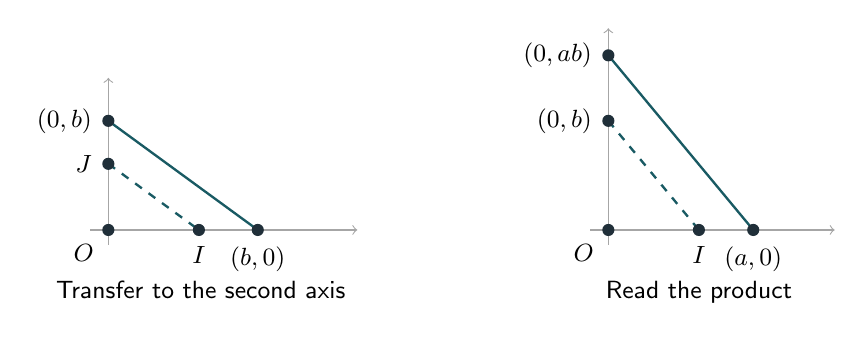
\begin{tikzpicture}[x=1.15cm,y=.84cm,font=\small,
  axis/.style={->,gray!70}, drawline/.style={line width=.85pt,color=accent},
  pt/.style={circle,fill=ink,inner sep=1.55pt}]
\begin{scope}
  \draw[axis] (-.2,0)--(2.75,0);\draw[axis] (0,-.22)--(0,2.30);
  \draw[drawline,dashed] (0,1)--(1,0);
  \draw[drawline] (0,1.65)--(1.65,0);
  \node[pt,label=below left:$O$] at (0,0) {};
  \node[pt,label=below:$I$] at (1,0) {};
  \node[pt,label=left:$J$] at (0,1) {};
  \node[pt,label=below:{$(b,0)$}] at (1.65,0) {};
  \node[pt,label=left:{$(0,b)$}] at (0,1.65) {};
  \node[anchor=north,font=\sffamily\small] at (1.02,-.62) {Transfer to the second axis};
\end{scope}
\begin{scope}[xshift=6.35cm]
  \draw[axis] (-.2,0)--(2.50,0);\draw[axis] (0,-.22)--(0,3.05);
  \draw[drawline,dashed] (0,1.65)--(1,0);
  \draw[drawline] (0,2.64)--(1.6,0);
  \node[pt,label=below left:$O$] at (0,0) {};
  \node[pt,label=below:$I$] at (1,0) {};
  \node[pt,label=below:{$(a,0)$}] at (1.6,0) {};
  \node[pt,label=left:{$(0,b)$}] at (0,1.65) {};
  \node[pt,label=left:{$(0,ab)$}] at (0,2.64) {};
  \node[anchor=north,font=\sffamily\small] at (1.00,-.62) {Read the product};
\end{scope}
\end{tikzpicture}
\caption{Multiplication in the recovered field. In each diagram the solid line
is parallel to the dashed line. The transfer construction moves the final
ordinate back to the baseline. The formulas also cover zero and negative
inputs.}\label{fig:intercept}
\end{figure}


Define $R(z)$ by $B(O,z,I)\lor B(O,I,z)$, and define
$x\preceq y$ by $\exists z\,[A(x,z,y)\land R(z)]$. For
$z=O+c u$, the first disjunct gives $0\le c\le1$, the second gives
$1\le c$, and their union gives $c\ge0$. This recovers the directed
order on the whole baseline. Additive inverse and division by a nonzero
scalar have unique graphs from addition and multiplication. When a total
reciprocal is part of the scalar language, assign reciprocal zero at zero.

\subsection{The two inverse maps}

\paragraph{Framed interpretation theorem.}
For every decidably linearly ordered field $F$, constructing its
point plane and interpreting the baseline recovers an isomorphic ordered
field. Constructing the point plane of that baseline recovers a point
structure isomorphic to the original framed plane. Both isomorphisms
have explicit graphs. For a primitive recursive presentation of $F$
with decidable equality, order and primitive recursive totalized
division, the two isomorphisms on codes are primitive recursive.

\emph{Proof.}
The scalar isomorphism is $a\mapsto O+a u$ by the four computations
above. For the point isomorphism use $G$. Its inverse sends a point
$Q$ to the two baseline points indexed by
\[
 a=\frac{(Q-O)\cdot u}{N},\qquad
 b=\frac{(Q-O)\cdot v}{N}.
\]
Indeed, the difference $Q-O-au-bv$ is orthogonal to both basis vectors
and hence zero by the nonzero determinant. For any two such points their
squared distance in the original plane equals
$N((a_1-a_2)^2+(b_1-b_2)^2)$. Since the factor $N>0$ is common to all
segments, congruence is preserved and reflected. Affine interpolation
commutes with the coordinate map and its inverse, preserving and
reflecting inclusive betweenness. The maps carry the three named points
to the canonical frame. The displayed expressions use a fixed finite
number of field operations and one division by a proved positive
element. On a coded field each step respects code equality. This also
supplies the asserted primitive recursive implementations.\hfill$\square$

For example, testing which side of a directed line a point lies on
uses the sign of a determinant after a frame has been chosen. Reversing
the orientation of the frame reverses this sign. Equidistance and
betweenness survive every frame change, including a common change in the
length unit. Naming the frame specifies the scalar identification used
in the theorem.

\subsection{An intrinsic point-only axiomatization}

There is a direct way to state the scope of the inverse theorem for
abstract structures. Let $\mathcal F$ be a first-order theory of
decidably linearly ordered fields. For example it may require square
roots of all positive elements, or in addition roots of every odd-degree
polynomial. The latter choice gives real-closed ordered fields. Form a
point theory with $B,\equiv,O,I,J$ by imposing the following explicit
axioms. Every mention of $H,K,S,A,P,G$ abbreviates the point formulas
above.
\begin{enumerate}
\item The named triple satisfies the frame formula. On $H$, the graphs
$A,P$ are everywhere defined and single-valued. With constants
$O,I$, operations so defined, and relation $\preceq$, the relativized
axioms of $\mathcal F$ hold.
\item For every $Q$ there is exactly one pair $(x,y)\in H^2$ with
$G(Q;x,y)$, and for every such pair there is exactly one $Q$.
Here quantification over a pair means two ordinary point quantifiers.
\item For points with coordinates supplied by $G$, congruence is equality
of the two squared distances in $H$. For coordinate pairs $a,b,c$,
$B(a,b,c)$ is equivalent to
\[
 \det(b-a,c-a)=0\quad\land\quad(b-a)\cdot(b-c)\le0 .
\]
Both are fixed polynomial tests over the interpreted field, hence
first-order point formulas using the graphs of arithmetic.
\end{enumerate}
To check the betweenness test, if $a=c$ the inequality forces $b=a$
by nonnegativity of squares. Otherwise the determinant supplies
$b=a+t(c-a)$ by division along a nonzero component. The inequality is
$t(t-1)\|c-a\|^2\le0$, equivalently $0\le t\le1$. Thus all three
axioms hold in the plane of every field satisfying $\mathcal F$.

Conversely, in any point structure satisfying this list the interpreted
baseline is a model of $\mathcal F$ by item 1. Item 2 supplies the graph
of an isomorphism onto its coordinate plane, and item 3 verifies both
directions on each primitive predicate. To see that the named frame is preserved,
item 3 first makes the coordinate map an isomorphism of unframed point
structures, and therefore carries the original defining formulas to the
same formulas in an actual field plane. There the calculations above
give $G(O;O,O)$, $G(I;I,O)$ and $G(J;O,I)$ (with the frame and scalar
points carried along by that map). Pulling these formulas back gives
the assertion in the original structure. This proves a two-sided
first-order interpretation for the stated presentation. Uniquely
defined operations may equivalently be retained as graphs throughout,
so the proof requires no choice of representatives or choice principle.
For the point language without named constants, the same formulas
give an interpretation with a frame as parameter.

The list is a coordinatization axiom presentation in point language.
Its algebraic and geometric content is explicit. A representation theorem
for a separately chosen synthetic axiom system with intuitionistic logic
would require deriving the list from that system. The inverse theorem here
applies directly to the stated presentation and to the exact plane used
in this report.

\paragraph{Checked Lean component.}
\texttt{FrameRelations.lean} defines the point-language graphs.
\texttt{CanonicalFrame.lean} proves the transfer, addition, multiplication,
order and coordinate formulas in the standard frame over every linearly
ordered field, and proves that the coordinate graph is a bijection.
Its executable algebraic test for $B(A,M,D)$ uses collinearity together
with $|AM|^2\le |AD|^2$ and $|MD|^2\le |AD|^2$.
For unequal endpoints the parameter $t$ converts these inequalities to
$t^2\le1$ and $(1-t)^2\le1$. Their conjunction is precisely
$0\le t\le1$. Equal endpoints force $M=A$. The file verifies that
equivalence, so its point predicates agree with those above. The Lean
results concern the field semantics. The interpretation of the underlying
arithmetic in iPRA is a separate part of the argument.

\section{Straightedge, compass and a nine-point circle}
\label{sec:constructions}
A line is given by $(A,u)$ with $N(u)>0$ and consists of $A+tu$.
This is an extensional representation: two such records describe the same
line precisely when their directions are proportional and one base point
lies on the other line. A circle $(C,s)$ uses its squared radius $s\ge0$,
with equation $N(X-C)=s$; $s=0$ gives a single point.
Every line can also be specified by two distinct points; every
circle can be specified by its center and a point on it.
All choices in the following classification are made on exact codes.

\paragraph{Two lines.}
For $A+tu=B+hv$ put $d=[u,v]$. If $d\ne0$, crossing with $v$
gives $t=[B-A,v]/d$ and crossing with $u$ gives $h=[B-A,u]/d$.
The two coordinates agree because their difference has zero cross
product with each vector of a basis. This proves existence and uniqueness.
If $d=0$, compare $[B-A,u]$ to zero to distinguish equality of lines
from disjoint parallel lines. The unique parallel to $(A,u)$ through $X$
is $(X,u)$, and its unique perpendicular there is $(X,Ju)$:
the solutions of $w\cdot u=0$ are the multiples of $Ju$.

\paragraph{A line and a circle.}
The foot from $C$ to $(A,u)$ is
\[
        F=A+u\frac{(C-A)\cdot u}{N(u)} .
\]
Indeed $F$ belongs to the line and $(C-F)\cdot u=0$; subtraction
gives uniqueness. For any point $F+tu$ on the line,
$N(F+tu-C)=N(F-C)+t^2N(u)$. Put $d=s-N(F-C)$.
There are zero, one or two intersections according as $d<0$, $d=0$
or $d>0$. They are $F$ at tangency and
$F\pm u\sqrt{d/N(u)}$ in the secant case. These exhaust the
solutions since $t^2=a^2$ implies $t=a$ or $t=-a$ in this field with decidable equality.
The formulas include the point-circle case.

\paragraph{Two circles.}
For $(C,s),(D,t)$ put $u=D-C$. If $u=0$, equality of squared radii
gives the same locus; different radii give disjoint loci. An identical
point-circle has just its center; an identical positive-radius circle
is returned as a whole circle. If $N(u)>0$, subtract the equations.
Every common point is on the line
\[
 C+k u+hJu,\quad k=\frac{N(u)+s-t}{2N(u)},\quad h\in K.
\]
Indeed this line is precisely the solution of
$2(X-C)\cdot u=N(u)+s-t$. Its substitution in the first circle gives
$h^2=s/N(u)-k^2$. The sign and square root give the exact number and
coordinates as in the preceding construction. Any candidate satisfying
the first circle and the subtraction satisfies the second circle.
All tests, including tangency, are primitive recursive.

\paragraph{Which of these witnesses can be drawn?}
Fix a frame with unit length and initial points. Let $E_0$ be the
subfield of $K$ generated by their coordinates in that frame.
Allow an intersection of already specified objects to return one of
its finitely many points, with either choice allowed. Parallel and
perpendicular constructions can be done with the two instruments.
For a perpendicular through $X$ to line $AB$, try the circles centered
at $X$ through $A$ or $B$. At least one gives a secant, since only the
foot on the line can give a tangent or a point-circle with its center on
the line. Its two intersection points have a perpendicular bisector
through $X$. To draw that bisector, use circles centered at the two
points through each other. Their two intersections lie on the bisector
and are distinct (their height squared is three quarters of the squared
chord length). Drawing two perpendiculars gives a parallel. Intersect
the bisector with the chord to obtain its midpoint. Equal input points have their common point as midpoint.

A point is obtainable by a finite construction exactly when both its
coordinates belong to the union of finite towers
\[
 E_0\subseteq E_1\subseteq\cdots\subseteq E_n,
 \qquad E_{i+1}=E_i(\sqrt{a_i}),\quad a_i\in E_i,\quad a_i>0.
\]
For necessity use the intersection formulas at each instruction.
For sufficiency, the constructions of Section~\ref{sec:frame-inverse}
realize addition and multiplication on the baseline. In detail, to copy
a displacement from $A$ to $D$ onto $C$, reflect $A$ through the midpoint
of $D,C$; if $A$ is that midpoint, return it. Otherwise the line
through $A$ and the midpoint and the circle about the midpoint through
$A$ give the other endpoint. The transfer diagram uses a parallel through
the input and its intersection with the other axis; the direction has
a nonzero transverse component. The coordinates of each initial point are obtained by parallels to the axes and this transfer in reverse. The product uses a parallel to the line
from $(1,0)$ to $(0,b)$, so it is also defined for $a=0$ or $b=0$.
Reflecting through the origin gives the negative. For $b\ne0$,
use the parallel through $(0,1)$ to the direction $(-1,b)$;
it meets the baseline at $(1/b,0)$. To construct $\sqrt a$, intersect
the vertical axis with the circle having diameter $(-1,0),(a,0)$.
At abscissa zero the circle equation is $y^2=a$; take the nonnegative
point and transfer its ordinate. Finally combine a horizontal and a
vertical displacement. A finite tower consists of field expressions
with finitely many such square roots since adjoining a root adjoins all
quotients of polynomial expressions in it. Two towers can be concatenated
with their radicands read in the enlarged intermediate fields.
This proves the stated characterization. It concerns generated finite
constructions with no arbitrary extra input points.

For example $T^3-2$ has a positive root in $K$. Over the unit rational
frame it cannot be drawn by these instruments. A rational root of the
monic integer cubic would have to be an integer divisor of $2$, and
none is a root, so its degree is three. Each tower step has degree one
or two, by reduction modulo $T^2-a_i$; when no square root is present
the quadratic is irreducible. Multiplying dimensions along finite field
extensions is justified by taking products of bases. Hence a degree-three
subfield cannot occur in such a tower, since three cannot divide a
power of two. The formula demanding a cube root is expressible with
points by the framed product graph. Its witness illustrates precisely
what the first-order completion adds to straightedge and compass.

\subsection{A theorem using incidence, length and construction}
\begin{proposition}[The nine-point circle, including right triangles]
For every noncollinear triangle the three side midpoints, the three
altitude feet and the three midpoints from its vertices to the
orthocenter lie on one explicitly constructible circle. Its radius is
half the circumradius.
\end{proposition}
\begin{proof}
The perpendicular bisectors of $AB$ and $AC$ have independent directions,
since $B-A,C-A$ do. Their unique intersection $O$ is equidistant from
all three vertices, and is their unique circumcenter. Translate $O$
to the origin; write the vertex vectors as $a,b,c$ with common norm
length $R>0$. Put $h=a+b+c$. Then
$(h-a)\cdot(c-b)=(b+c)\cdot(c-b)=0$; cycling proves that $h$ is on
each altitude. Two altitude directions are independent, so $h$ is their
unique common point. Put $n=h/2$. We will prove $|2p-h|=R$ for
each of the nine specified points $p$.

For $p=(b+c)/2$ one has $2p-h=-a$. For $p=(a+h)/2$ one has
$2p-h=a$. For the foot from $a$ to $bc$, let $m=(b+c)/2$ and
let $\Pi$ denote orthogonal projection on the direction $c-b$ through
zero. Because $m\cdot(c-b)=0$, the foot is $p=m+\Pi a$.
Thus $2p-h=2\Pi a-a$. The perpendicular summands $\Pi a$ and
$a-\Pi a$ have the same squared sum when the second is negated.
Consequently $|2\Pi a-a|=|a|=R$. Cyclic permutation proves the other
six assertions and gives $|p-n|=R/2$ throughout. The side midpoints
are noncollinear since their differences are half of two independent
side vectors, so the circle is unique. If the triangle is right several
of the nine points coincide; the argument only used nonzero side
lengths and a nonzero triangle determinant.
\end{proof}

The same determinant measures area: the oriented area of $ABC$ is
$[B-A,C-A]/2$. Splitting at any $X$ replaces this expression by the sum
for $XBC,AXC,ABX$ by bilinearity and alternating signs. Consequently a
triangulated polygon has signed area one half of the sum of
$[P_i,P_{i+1}]$ on its oriented boundary: the two opposite orientations
of each internal edge cancel. This definition uses only a finite sum.

\section{Rigid motions and congruence of finite figures}
\label{sec:motions}
Let $J(x,y)=(-y,x)$ and write $[u,v]=u_1v_2-u_2v_1$.
Every distance-preserving map of the plane has the form
$X\mapsto t+UX$ for an orthogonal $2\times2$ matrix $U$. To prove this,
subtract the image of the origin, and call the resulting map $f$. The
vectors $u=f(1,0)$ and $v=f(0,1)$ have squared length one and squared
distance two, hence $u\cdot v=0$. For $X=(a,b)$, subtraction of its
squared distances to the origin and to $(1,0)$ gives
$f(X)\cdot u=a$. Comparison with $(0,1)$ similarly gives
$f(X)\cdot v=b$. Since $u,v$ form an orthonormal basis, $f(X)=au+bv$.
Conversely every displayed map preserves squared distances, has inverse
$Y\mapsto U^{\mathsf T}(Y-t)$, and preserves betweenness. Thus motions
can be represented by six scalar entries subject to $U^{\mathsf T}U=I$.
Assertions about such motions are first-order field assertions. The
argument about an arbitrary map is a schematic statement about a map
supplied in the metatheory; the finite code suffices inside arithmetic.

\begin{proposition}
Two labelled lists $P_1,\ldots,P_n$ and $Q_1,\ldots,Q_n$ are congruent by
a rigid motion, allowing reflection, if and only if all corresponding
pairwise squared distances agree. There is a PR procedure computing a
motion or returning a mismatched pair.
\end{proposition}
\begin{proof}
Compare all pairs. Necessity follows from the definition of motion.
For the converse, return the identity for empty lists. If all $P_i$
coincide, all $Q_i$ coincide, and translation by $Q_1-P_1$ works.
Otherwise choose a distinct pair, renumbered as $1,2$. Put
$u=P_2-P_1$, $v=Q_2-Q_1$, and $N=u\cdot u=v\cdot v>0$.
Write
\[
   P_i=P_1+a_i u+b_i Ju,\qquad Q_i=Q_1+c_i v+d_i Jv .
\]
The coefficients are dot products with the basis vectors divided by
$N$. Distances to points $1,2$ give $a_i=c_i$ by subtraction and then
$b_i^2=d_i^2$ from the distance to point $1$. If every $b_i=0$, every
$d_i=0$ and take $e=1$. Otherwise choose $k$ with $b_k\ne0$. Set
$e=d_k/b_k$, so $e^2=1$. Expanding the distance between points $i,k$
and using the known squares gives $b_i b_k=d_i d_k$. Dividing by $b_k$
and multiplying by $e$ yields $d_i=e b_i$ for all $i$. In both cases a
witness is the map
\[
 P_1+au+bJu\ \longmapsto\ Q_1+av+e bJv .
\]
The basis pairs are orthogonal and have common squared length $N$, so
this map is a rigid motion. Its determinant is $e$. In the collinear
case either sign works. In the noncollinear case the two basis
coefficients at $k$ force the sign, so this also decides congruence by
orientation-preserving motions. Every search ranges over a given finite
list.
\end{proof}

The pure point language records equidistance and leaves the unit of
length free. Its automorphisms on the real algebraic plane are exactly
the similarities, including those reversing orientation. Indeed, an
automorphism sends any frame to a frame, and the relational definitions
of Section~\ref{sec:frame-inverse} make its induced map on numerical
coordinates an ordered-field automorphism. Such an automorphism fixes
each rational and thus fixes each real algebraic number. The unique
zero of its record polynomial in its rational isolating interval
must go to the same zero. Consequently the point map is exactly the
frame change $O+au+bv\mapsto O'+au'+bv'$. Its linear part multiplies
all squared distances by the common positive factor
$(u'\cdot u')/(u\cdot u)$. Conversely these similarities preserve
betweenness and congruence, as follows directly from those formulas.

For unlabelled finite configurations of the same cardinality, enumerate the
permutations of the second list and apply the labelled procedure in order.
The first success gives both a matching and a witnessing motion. Conversely
any congruence of the configurations induces a permutation on the listed
points (with multiplicities matched if the lists describe multisets).
Exhausting the $n!$ possibilities therefore certifies failure.

\section{What happens to the continuum?}
Every real algebraic point is a genuine Euclidean point. The embedding
$K^2\hookrightarrow\mathbb R^2$ preserves and reflects \emph{every}
first-order point formula on its parameters, by Theorem~\ref{thm:transfer}.
This property is called an elementary embedding. In the standard model
$K$ is itself Archimedean: read the coarse enclosure of $x$ and take an
integer exceeding its endpoints in absolute value. For $x<y$ the exact
sign algorithm provides a positive rational lower bound on the gap;
sufficiently fine rational reads give disjoint intervals with a rational
between them. This proves rational density constructively.

Completion nevertheless changes the individual points. Externally, finite
codes are countable, whereas the points of a real line are uncountable.
For a concrete second-order distinction take a transcendental real $t$.
The external subset $\{a\in K:a<t\}$ has no supremum in $K$. A proposed
supremum $s<t$ is too small by rational density, and for $s>t$ there
is a smaller rational upper bound. The remaining equality would make
$t$ algebraic. This subset cannot be first-order definable over $K$ with
algebraic parameters, since the one-variable cell argument gives a
supremum for each inhabited bounded definable subset.

\paragraph{A separate presentation for approximations.}
One can work over a real coordinate specified by a particular PR family
of nested rational intervals $[l_n,r_n]$ of width at most $2^{-n}$.
Such specifications may carry free numerical parameters. Coordinate
equality means agreement at every precision. A strict sign has a
positive separation witness. In this setting affine combinations, dot
products, projections with a supplied lower bound on $N(u)$, and
well-separated line intersections retain effective meanings. For example,
for $d=[u,v]$ with $|d|\ge\eta>0$, an enclosing interval for $d$
of width $<\eta/2$ has distance at least $\eta/2$ from zero. Reciprocal
then magnifies interval widths by at most $4/\eta^2$. Applying the
sum and product width bounds of Section~\ref{sec:scalar} to
$A+u[B-A,v]/d$ gives a PR request for input precisions at any desired
output precision. Each fixed finite construction is handled by passing
accuracy requests backwards along its operation list. At exact tangency
the intersection point itself may still be given; a uniform test for the
number of intersections has a different computational requirement.

For a proof, fix an effective enumeration of machines on empty input.
Bounded simulation for $n$ steps is primitive recursive in the machine
index and $n$. If the first halt occurs at step $t\le n$, let
$I_{e,n}=[2^{-t},2^{-t}]$. Otherwise let $I_{e,n}=[0,2^{-n}]$.
These are nested, have the required width, and represent a scalar
$x_e$ equal to zero exactly when machine $e$ never halts. A uniform
effective test for equality of all such names would decide the halting
problem. Briefly, a halting decider on machines and inputs would allow a
machine on input $k$ to halt just when machine $k$ on input $k$ is
predicted to run forever; applying this to its own index contradicts
either prediction. Compiling any fixed input into an empty-input
machine transfers that impossibility to the present enumeration.
All the individual $x_e$ are even rational in the classical metatheory.
What fails is uniform conversion of these names to exact algebraic comparison
data. Geometrically, the unit circle and horizontal line $y=1+x_e$ are
tangent exactly in the zero case and disjoint otherwise. This shows why
the choice of input representation matters even to an elementary
construction. See Beeson's analysis of uniform geometric constructions
for the different role of continuity in synthetic constructive geometry
\cite{beeson}.

\section{Lean development and the remaining object proofs}
\label{sec:lean}
The repository uses \texttt{PR k} for $k$-ary primitive recursive function
\emph{syntax}, \texttt{PTm n} for terms with $n$ free numerical variables,
\texttt{Fm PTm n} for formulas, and \texttt{Prf PRAAx} for their
derivations~\cite{proveit}. An assertion proved in Lean about a
\texttt{Field} differs in type from a derivation in this embedded theory.
The archive contains examples of both. The distinction determines which
steps can already be imported.

\subsection{What the included Lean modules prove}
\begin{description}[leftmargin=0pt,labelsep=0pt,labelwidth=0pt,style=nextline]
\item[\texttt{MetricIdentities.lean}.]
\texttt{gramClosed} and \texttt{midpointClosed} are closed embedded
iPRA derivations. Each of four integer coordinates is encoded by a
difference of two natural variables. The first proves
$N(u)N(v)=(u\cdot v)^2+[u,v]^2$. The second proves the parallelogram law
$N(u+v)+N(u-v)=2N(u)+2N(v)$. The universal closures have eight
natural binders. The open versions allow substitution of arbitrary
integer terms in an arbitrary context. These endpoints use the repository's
\texttt{ZT.derive}, \texttt{ipra\_ring} and \texttt{closeUniv}.
This is precisely the polynomial part of the length and frame arguments.
Transferring the identities to scalar records also needs their field laws.
\item[\texttt{Translation.lean}, \texttt{Axioms.lean} and \texttt{Bridge.lean}.]
The first module defines the two formula languages, term evaluation,
environments, shadowing and the quantifier translation. Its
\texttt{translate\_correct} proves preservation and reflection for every
formula. The second module works over a linearly ordered field; it
proves the equivalence of affine betweenness and the determinant/dot
test, inner Pasch, the Euclidean axiom and five segments. The bridge
composes these proofs using an independent affine interpretation.
\texttt{translated\_innerPasch} checks the closed translated sentence
including the existential point binder.
\item[\texttt{FrameRelations.lean} and \texttt{CanonicalFrame.lean}.]
The first defines all point-language construction graphs. Its
\texttt{BiGraph} explicitly carries the four existence/uniqueness clauses
for a relational bijection and gives both round trips and quantifier
transport. The second proves the midpoint and collinearity criteria for
a concrete Cartesian plane over a linearly ordered field, the equivalence
of its betweenness test with affine interpolation, the standard-frame
addition, multiplication and order formulas, and the coordinate bijection.
The arbitrary-frame formulas in Section~\ref{sec:frame-inverse} are written
as mathematical proofs.
\item[\texttt{ObjectLanguage.lean}.]
This compiler takes seven PR symbols (validity, the scalar zero, three
ring operations, equality and order) and sends the translated language
to actual \texttt{Fm PTm n}. Under binders it shifts older terms and
guards the new variable; it interprets both scalar tests by the Boolean
numeral one. \texttt{closeTranslation} yields an exact type of sentence
for a closed point formula once the symbols are filled. The scalar symbols
are an explicit input to this file.
\end{description}
The included Lean files were compiled using Lean and mathlib 4.32.0.
The two closed object proofs print the standard Lean metatheoretic
dependencies \texttt{propext}, \texttt{Classical.choice} and
\texttt{Quot.sound}. Their values inhabit \texttt{Prf PRAAx};
the constructors of that inductive calculus fix the available
object axioms. The general scalar presentation and the elimination
theorem here have human proofs; their complete object-calculus proof
generators remain to be implemented.

\subsection{A route to closing the general theorem}
Here is an implementation order and the statement to verify at each step.
All semantic equalities between two codes in these obligations abbreviate
the numerical Boolean predicate for equality of their values.
\begin{enumerate}
\item \emph{Arithmetic and records.} Use the upstream
\texttt{Core/Pairing}, \texttt{Core/Division}, \texttt{Core/Gcd},
\texttt{Core/Order}, \texttt{Core/Search} and \texttt{Core/Definitions}
for pairs, bounded loops and simultaneous recursion. Pick one list format,
for example the one in Section~\ref{sec:scalar}; use pairs for signed
numerators and positive denominators for rationals. Store a triple as
a list of length three. A normalized polynomial list has its final
coefficient nonzero unless it is empty. Define \texttt{valid}, interval
reading and every guard by the exact rational tests in
\eqref{eq:intervalcheck}. Encode the recipe to read a record as a
single PR function of the record and the precision. Prove nesting,
width and endpoint bounds by a Boolean invariant on the bisection counter.
For a bounded universal check, take the conjunction of the Boolean
values by recursion; prove its elimination and introduction lemmas once.
\item \emph{Scalar certificates.} Implement the finite convolution,
signed polynomial division, extended gcd and finite matrix determinant
with their coefficient-vector invariants. For each provisional operation
in the paper define its own fixed PR reader with parameters.
Prove the positive slope estimate, the sign gap, and the \emph{conversion}
lemma: the returned code is valid and agrees with the input recipe
at every precision. Prove agreement by fixing the precision before
induction and budgeting all intermediate reads. In the determinant
construction verify the adjugate coefficient identity by pairing
permutations; use it to certify the monic annihilator in the normalizer.
Prove validity, extensionality, field laws and order laws for
\texttt{add, sub, mul, eqTest, leTest}; add totalized inverse for use in
algorithms, keeping the ring language of the output compiler unchanged.
\item \emph{Root enumeration.} For a list $f$ of scalar coefficients
compute the tag for an identically zero polynomial or a strictly
increasing list $L_f$ of roots. The target on the finite-list branch is
$\mathrm{Valid}(x)\to(f(x)=0\leftrightarrow
     \bigvee_{i<|L_f|}x=L_f[i])$. Here the variable-size disjunction
is a bounded Boolean fold. The finite algebra and rational grid in
Section~\ref{sec:scalar} supply both inclusions. Polynomial IVT is a
separate witness theorem with two input signs; no appeal to a general
real-analysis library is needed.
\item \emph{One elimination.} Define signed remainders by a
degree-clocked loop. Define \texttt{query}, the sign counts
in~\eqref{eq:counts}, and the two tail signs. Prove~\eqref{eq:query}
by a finite sweep over the ordered roots from the preceding step.
The invariant is the integer equality between variation loss and root
contributions through the current cell. For a specialized polynomial
list, prove equivalence between each attainable sign condition and its
computed positive count or tail flag. Define \texttt{pick} from the actual
ordered point/interval samples to return a concrete satisfying code.
\item \emph{Reification and composition.} Generate the coefficient
decision tree with formal numerator/denominator pairs. At each node the
guard records every denominator needed to that point. For a fixed
matrix construct a \texttt{Prf} equivalence between an eliminated binder
and its disjunction of accepting branch guards, using \texttt{pick} on
a positive existential branch. Use the same witnesses for counterexamples
to universal claims. In the external proof generator recurse on a
particular syntax tree. Discharge its connectives by the natural
deduction constructors and the Boolean decision for its children.
For a closed sentence the final goal is a value of \texttt{Prf PRAAx []}
at the output of \texttt{closeTranslation}, or at its negation.
For parameters, universally close the valid-code guards and the
bi-implication with the decision bit. Only a completed object proof
is eligible for transport using the repository's \texttt{pra\_iff\_native}.
\end{enumerate}

The ProveIt packet \texttt{eight\_geometry\_theorems\_ipra} treats exact
rational/projective coordinate calculations with denominator guards.
Its approach applies to pieces such as the line-intersection formula.
The present development needs real algebraic coefficients for circle
intersections and the full first-order transfer. We reuse the repository's
checked arithmetic interface for the two embedded proofs.
The executable companions cover scalar records, exact constructions, the
one-variable signed-remainder computation, parameter-dependent elimination
for prenex polynomial formulas, and exact witness selection. The
optional symbolic routines use SymPy for rational polynomial arithmetic
and isolation. Their tests exercise the algorithms independently of Lean.

\paragraph{Further questions.}
How small can the proof generator for a single quantified sign test be
made using the repository's existing bounded-sum proofs? Can a
specialized compiler for ruler-and-compass statements avoid general
polynomial elimination while emitting comparable object-calculus
certificates? For analytic names, which operations admit continuous
computable selections through degeneracies after the input carries extra
orientation or separation data?

\begin{thebibliography}{9}
\bibitem{proveit} V.~Reshetnikov, \emph{ProveIt}, Primitive Recursive
Arithmetic, snapshot \texttt{83421593771f}.
\href{https://github.com/VladimirReshetnikov/ProveIt/tree/83421593771f877bc1ae98f4229eb35507bff05b/Logic/PrimitiveRecursiveArithmetic}{Repository and subdirectories}.
\bibitem{cm} C.~Cohen and A.~Mahboubi, \emph{Formal proofs in real algebraic
geometry: from ordered fields to quantifier elimination}, Logical Methods
in Computer Science 8 (2012).
\url{https://arxiv.org/abs/1201.3731}.
\bibitem{pr} D.~Perrucci and M.-F.~Roy, \emph{Elementary recursive
quantifier elimination based on Thom encoding and sign determination},
Annals of Pure and Applied Logic 168 (2017), 1588--1604.
\url{https://arxiv.org/abs/1609.02879}.
\bibitem{beeson} M.~Beeson, \emph{A constructive version of Tarski's
geometry}, \url{https://arxiv.org/abs/1407.4399}.
\end{thebibliography}
\end{document}
